%%%%%%%%%%%%%%%%%%%%%%%%%%%%%%%%%%%%%%%%%%%%%%%%%%%%%%%%%%%%%%%%%%%%
%% I, the copyright holder of this work, release this work into the
%% public domain. This applies worldwide. In some countries this may
%% not be legally possible; if so: I grant anyone the right to use
%% this work for any purpose, without any conditions, unless such
%% conditions are required by law.
%%%%%%%%%%%%%%%%%%%%%%%%%%%%%%%%%%%%%%%%%%%%%%%%%%%%%%%%%%%%%%%%%%%%

\documentclass[
  digital, %% This option enables the default options for the
           %% digital version of a document. Replace with `printed`
           %% to enable the default options for the printed version
           %% of a document.
  table,   %% Causes the coloring of tables. Replace with `notable`
           %% to restore plain tables.
  lof,     %% Prints the List of Figures. Replace with `nolof` to
           %% hide the List of Figures.
  lot,     %% Prints the List of Tables. Replace with `nolot` to
           %% hide the List of Tables.
  %% More options are listed in the user guide at
  %% <http://mirrors.ctan.org/macros/latex/contrib/fithesis/guide/mu/fi.pdf>.
]{fithesis3}
%% The following section sets up the locales used in the thesis.
\usepackage[resetfonts]{cmap} %% We need to load the T2A font encoding
\usepackage[T1,T2A]{fontenc}  %% to use the Cyrillic fonts with Russian texts.
\usepackage[
  main=english, %% By using `czech` or `slovak` as the main locale
                %% instead of `english`, you can typeset the thesis
                %% in either Czech or Slovak, respectively.
  english, czech %% The additional keys allow
]{babel}        %% foreign texts to be typeset as follows:
%%
%%   \begin{otherlanguage}{german}  ... \end{otherlanguage}
%%   \begin{otherlanguage}{russian} ... \end{otherlanguage}
%%   \begin{otherlanguage}{czech}   ... \end{otherlanguage}
%%   \begin{otherlanguage}{slovak}  ... \end{otherlanguage}
%%
%% For non-Latin scripts, it may be necessary to load additional
%% fonts:
\usepackage{paratype}
\def\textrussian#1{{\usefont{T2A}{PTSerif-TLF}{m}{rm}#1}}
%%
%% The following section sets up the metadata of the thesis.
\thesissetup{
    date          = \the\year/\the\month/\the\day,
    university    = mu,
    faculty       = fi,
    type          = mgr,
    author        = Bedřich Said,
    gender        = m,
    advisor       = {RNDr. Zdeněk Matěj, Ph.D.},
    title         = {//TODO},
    TeXtitle      = {//TODO},
    keywords      = {keyword1, keyword2, ...},
    TeXkeywords   = {keyword1, keyword2, \ldots},
    abstract      = {This is the abstract of my thesis, which can

                     span multiple paragraphs.},
    thanks        = {These are the acknowledgements for my thesis, which can

                     span multiple paragraphs.},
    bib           = example.bib,
}
\usepackage{makeidx}      %% The `makeidx` package contains
\makeindex                %% helper commands for index typesetting.
%% These additional packages are used within the document:
\usepackage{paralist} %% Compact list environments
\usepackage{amsmath}  %% Mathematics
\usepackage{amsthm}
\usepackage{amsfonts}
\usepackage{url}      %% Hyperlinks
\usepackage{markdown} %% Lightweight markup
\usepackage{listings} %% Source code highlighting
\lstset{
  basicstyle      = \ttfamily,%
  identifierstyle = \color{black},%
  keywordstyle    = \color{blue},%
  keywordstyle    = {[2]\color{cyan}},%
  keywordstyle    = {[3]\color{olive}},%
  stringstyle     = \color{teal},%
  commentstyle    = \itshape\color{magenta}}
\usepackage{floatrow} %% Putting captions above tables
\floatsetup[table]{capposition=top}

\begin{document}

\chapter{Introduction}
//todo

\chapter{Hardware}
The hardware design is split into several steps in this paper. First, I had to decide if it's really necessary to build a new device or if I can find a suitable solution on the market. When we want to select a suitable device for our task, we have to know the specification of the task itself. The task is specified in section \ref{HWtaskAnalysis}. Based on the task we can specify all requirements that the selected device should meet (section \ref{HWrequirements}). Now, we can start looking for a device that fulfills all the requirements (section \ref{HWavailableSolutions}).

When we don't find any suitable device on the market, we can start to think about creating a new one. In my opinion, it's not a good way to start any development before doing the previous steps.

When we already start a development of a new hardware we can think about adding some additional requirements for increasing the versatility of the final hardware. Of course, the new requirements mustn't rapidly increase the final prize. But if the hardware will be used only in the specific task, it's usually unnecessary to add any other functionality. In this case, I'm adding some additional requirements in section \ref{HWadditionalRequirements}, because I think that in this case, I can add very high versatility with very low additional cost. The analysis of the final expenses is in section \ref{HWadditionalCosts}.

When I'm decided to develop a new hardware and I have the specification of all the requirements, I can start the development process. The selection of chips and other parts is in section \ref{HWdeviceSelection} and the printed circuit board (\ac{PCB}) design is discussed in section \ref{HWpcbDesign}.

Finally, the manufacturing of the first prototype is described in section \ref{HWmanufacturing}. With the first prototype, it's time for testing. The tests should find as many errors as possible and they should proof us if the requirements were already met. The section \ref{HWtesting}. The whole process is shown in the figure \ref{fig:HWprocess}.

\begin{figure}
	\centering
	\label{fig:HWprocess}
	\caption{Flowchart of the hardware design process}
	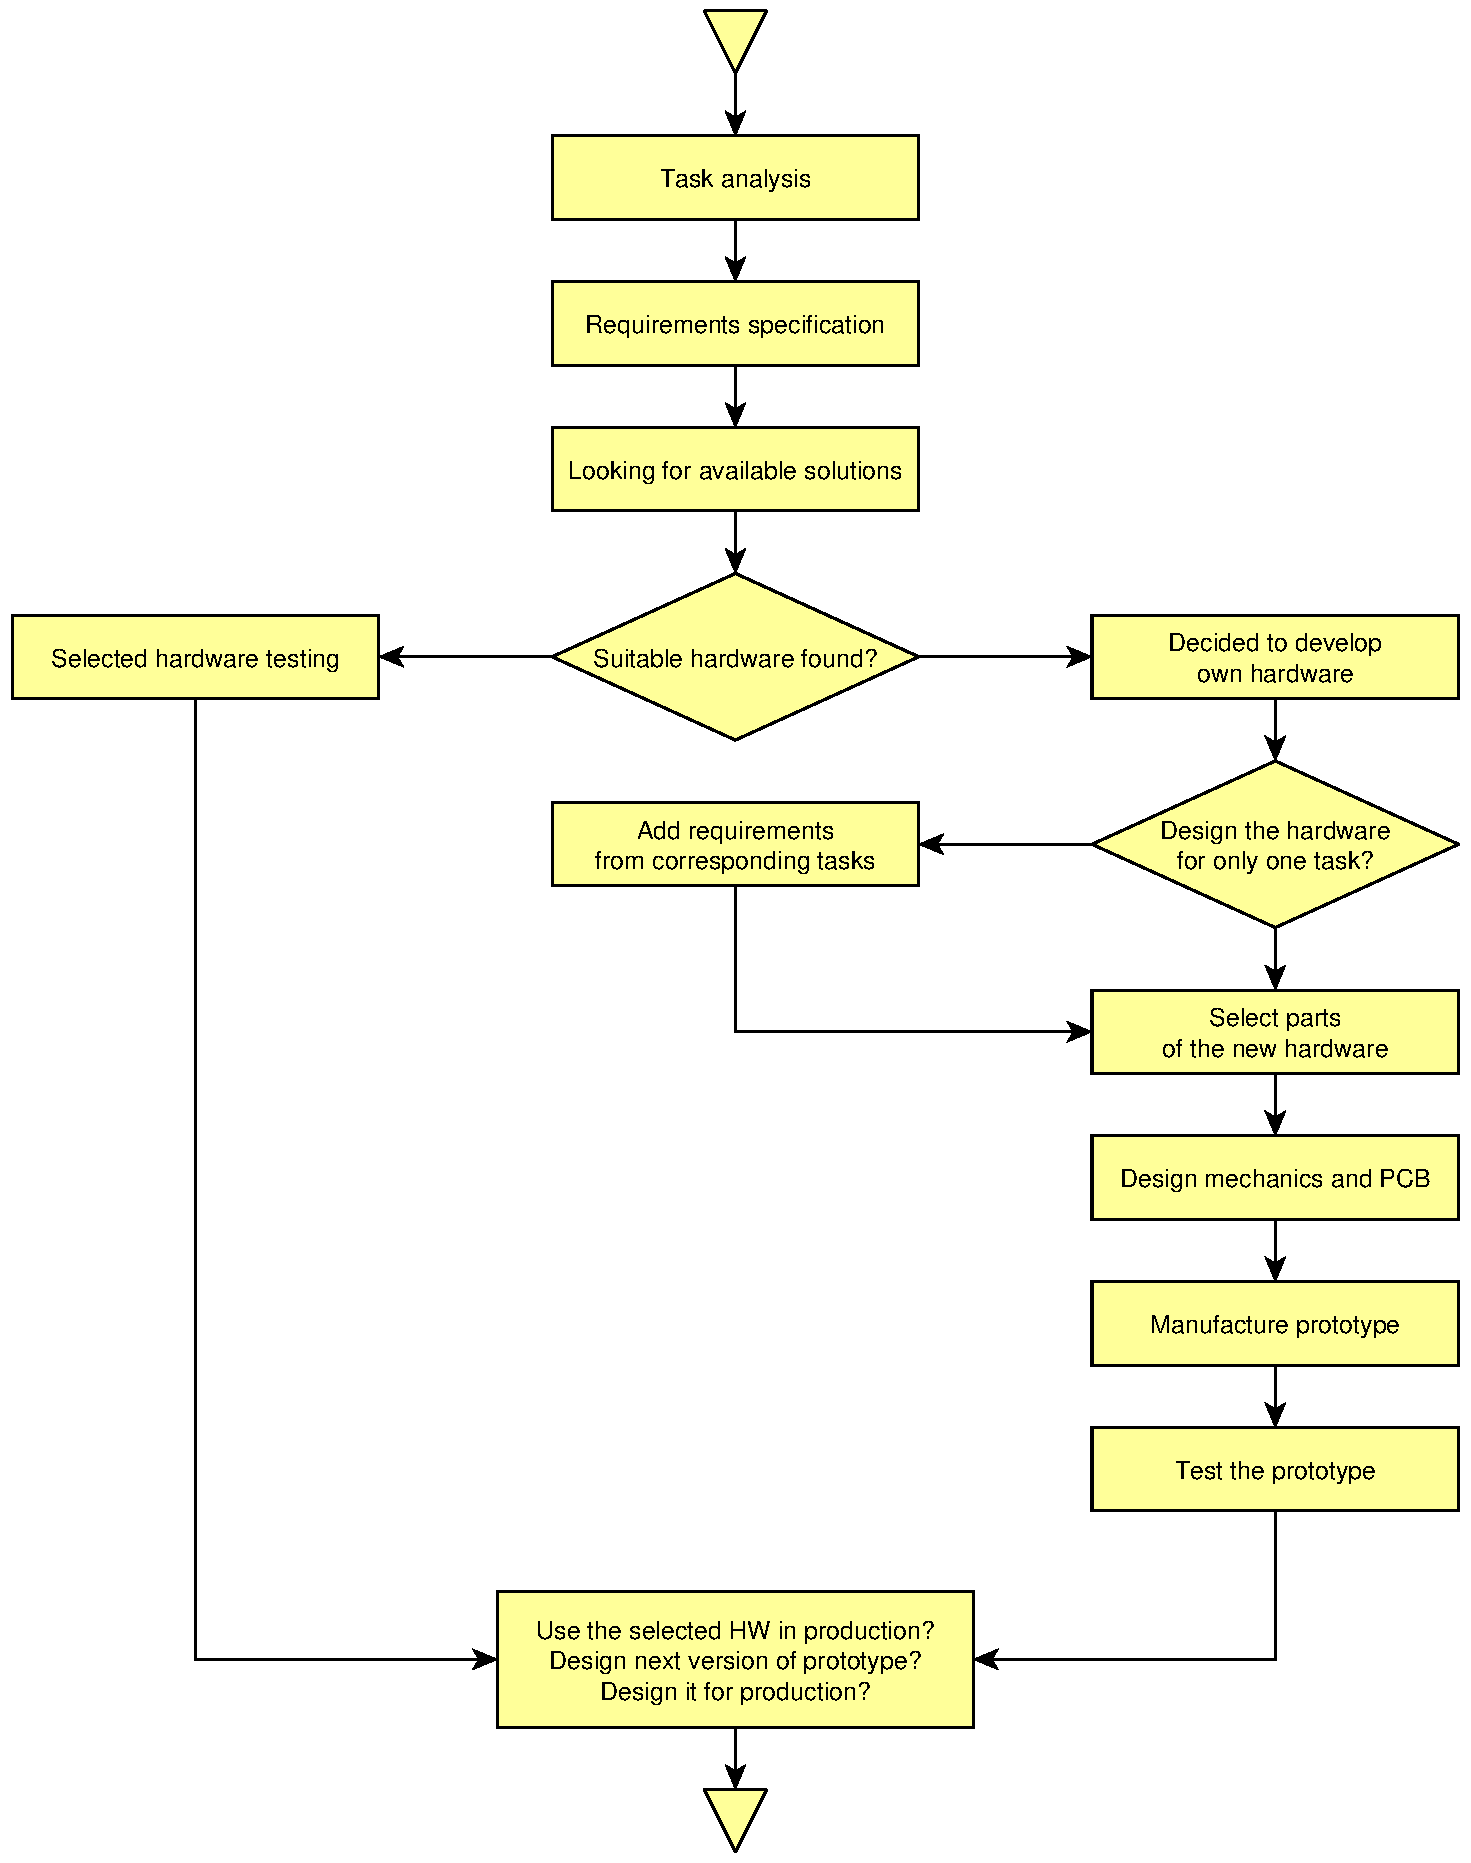
\includegraphics[width=\linewidth]{img/HWdesignProcess.pdf}
\end{figure}

\section{Task Analysis}
\label{HWtaskAnalysis}
When we define our complete task in the first step, then we can derive all requirements for our solution. Finally, we can check if our project was successful based on the previously defined task and requirements.

\highlightedBox{Movement analysis task description}{
	\begin{enumerate}
		\item Measuring of the movement of a subject
		\item Logging the measured data and sending them to post-processing
		\item Analysing of the movement and naming the specific categories of movements
	\end{enumerate}
}

The subject is an animal -- horse in this paper -- or human being or a moving machine. The post-processing can be done real-time during the measurement process, but this is not mandatory. The analysis is primarily focused to recognize known movements in logged data. For example, the categories of movement of a horse are stand, walk, trot, gallop, \dots

\section{Requirements}
\label{HWrequirements}
The development of a new hardware or software is usually driven by specified requirements. In this paper, I have specified two groups of requirements. The first group is based on the selected task to solve. The second group has lower priority and specifies all the requirements that I found during other similar tasks with similar hardware. The second group of requirements is adding higher versatility to the final electronic device with very low additional cost. These two groups of requirements are later merged and used as a source for next development of the hardware.

\subsection{High level requirements}

\paragraph{Measuring of the movement of a subject:} The solution should work outdoor. So, we cannot take into account any studio or laboratory-based technologies like Motion Capture (Mo-cap). On the other hand, we can replace the passive or active markers with the whole sensors and remove the necessary cameras. The sensor-based electronics is easier to install and can be used in large and complex areas. Based on this outdoor requirement I will consider only wearable sensor systems.

\paragraph{Logging the measured data and sending them to post-processing:} There are no wires acceptable for outdoor use, so we can log the data to internal memory or transmit them via any wireless technology. The wireless systems may be not fully reliable in complex areas with many objects. So, when we want to transmit the data directly it's still better to log them internally for later downloads.

\paragraph{Analysis of the movement and naming the specific categories of movements} This is a software requirement, so it's not very important during the hardware design. But this requirement defines what data we need to measure and this is a hardware requirement.

For the movement reconstruction, we primarily need data about position and attitude of every sensor. Some methods for movement classification don't need to know the exact location (for example accelerometer-based step counter). This task is focused on developing a new analysis of the movement, so now I cannot exactly say what sensors will be needed in the future. I can make a prediction that the inertial measurement unit (\ac{IMU}) and some location sensors will be needed. But there are some other sensors that produce interesting data according to the movement analysis, for example, a heart rate sensor according to animals.

Finally, I would like to add as many interesting sensors as possible, because it will give us more data sources and we are less limited by the data sources. The other advantage is multifunctionality of the hardware. On the other hand, these additional sensors should be added only into additional requirements with lower importance. Otherwise, the selection of an appropriate hardware (based on the requirements) will be manipulated by a number of probably unnecessary sensors.

\subsection{Low level requirements}
Finally, I've chosen a wearable sensors technology. The next requirements are specific to this technology and focused on the selection of the devices. Let's call a used wearable device or devices as Sensor Board. The table \ref{tab:requirements} shows the list of requirements for this Sensor Board.

\begin{table}
	\centering
	\caption{Sensor Board low level requirements 1}
	\label{tab:requirements}
	\begin{tcolorbox}[tab2,tabularx={X|p{12cm}},title=Importance legend]
		\greenLow    & Nice to have \\
		\yellowMedium & Very useful, reduce time or human effort \\
		\redHigh & Mandatory, impossible without this functionality \\
	\end{tcolorbox}
	\vspace{1cm}
	\begin{tcolorbox}[tab2,tabularx={|c|X|c|},title=Low level requirements 1]
		Category & Requirement & Importance \\ \hline \hline
		
		& Accumulator & \redHigh \\
		& Battery percentage indicator & \redHigh \\
		& Charging when external power applied & \redHigh \\
		& Voltage and current sensor & \yellowMedium \\
		& Power LED & \redHigh \\
		& Power switch & \redHigh \\
		& Automatic selection between external and battery power & \redHigh \\
		\multirow{-8}{*}{Power Supply} & Standardized charging connector & \yellowMedium \\ \hline
		
		& Accelerometer & \redHigh \\
		& Dynamic Gyroscope & \redHigh \\
		& Magnetometer & \redHigh \\
		& Indoor position & \yellowMedium \\
		& Outdoor position & \greenLow \\
		& Barometer & \greenLow \\
		\multirow{-7}{*}{Sensors} & Board temperature & \greenLow \\ \hline
		
		& Allow user programming & \redHigh \\
		& Wireless programming & \greenLow \\
		& Wired programming & \redHigh \\
		& Wireless & \redHigh \\
		& Standardized protocol & \redHigh \\
		& Wired access & \redHigh \\
		\multirow{-7}{*}{Communication} & Connector for external sensors & \greenLow \\ \hline
	\end{tcolorbox}
\end{table}

\begin{table}
	\centering
	\caption{Sensor Board low level requirements 2}
	\label{tab:requirements}
	\begin{tcolorbox}[tab2,tabularx={|c|X|c|},title=Low level requirements 2]
		Category & Requirement & Importance \\ \hline \hline
		
		& Logging all data for several hours & \redHigh \\
		& Sensor fusion coprocessor & \greenLow \\
		\multirow{-3}{*}{Functions} & LED indicators & \redHigh \\ \hline
		
		& Wearable design & \redHigh \\
		& Dimensions under \SI{6}{cm} & \redHigh \\
		& Dimensions under \SI{3}{cm} & \greenLow \\
		& Weight under \SI{50}{g} & \redHigh \\
		\multirow{-5}{*}{Mechanical} & Weight under \SI{20}{g} & \greenLow \\ \hline
		
		& Control multiple devices simultaneously & \yellowMedium \\
		& Download logged data & \redHigh \\
		& Streaming data during measurement & \yellowMedium \\
		& Start logging on multiple devices by clicking one button & \yellowMedium \\
		& Time synchronization of multiple devices & \redHigh \\
		\multirow{-6}{*}{Software} & Possibility to upload data to a server & \redHigh \\ 
	\end{tcolorbox}
\end{table}

\subsection{Additional requirements}
\label{HWadditionalRequirements}
The additional requirements are shown in table \ref{tab:additionalReq}.

\begin{table}
	\centering
	\label{tab:additionalReq}
	\caption{Additional requirements for the SensorBoard}
	\begin{tcolorbox}[tab2,tabularx={X|p{12cm}},title=Importance legend]
		\greenLow    & Nice to have \\ \hline
		\yellowMedium & Useful, can significantly improve functionality \\ \hline
		\st{\redHigh} & Not applicable \\ \hline
	\end{tcolorbox}
	\vspace{1cm}
	\begin{tcolorbox}[tab2,tabularx={|c|X|c|},title=Low level additional requirements]
		Category & Requirement & Importance \\ \hline \hline
		& Coprocessor for periodic computations like sensor fusion & \greenLow \\
		& Piezo buzzer & \greenLow \\
		\multirow{-3}{*}{Functions} & Buttons & \yellowMedium \\ \hline
		
		& Ambient light & \greenLow \\
		& Humidity & \greenLow \\
		& Sound (microphone) & \greenLow \\
		\multirow{-4}{*}{Sensors} & Ambient temperature & \greenLow \\ \hline
		
		& UART, I2C, SPI connector & \greenLow \\
		& PWM outputs & \greenLow \\
		\multirow{-3}{*}{Communication} & Analog inputs & \greenLow \\ \hline
		
		Software & NMEA input & \greenLow \\ \hline
	\end{tcolorbox}
\end{table}

\section{Available solutions}
\label{HWavailableSolutions}
The table \ref{tab:availableSolutions} shows the overview of existing devices I have found.

\begin{table}
	\centering
	\caption{Available solutions}
	\label{tab:availableSolutions}
	\begin{tcolorbox}[tab2,tabularx={|X|c|l|p{8cm}|},title=Available solutions]
		Device & Link & Price & Main disadvantages \\\hline\hline
		
		MetaWear        & \cite{MetaWear} & \$ 80  & Low memory, impossible longer logging. Loosing packets during streaming. \\
		ArduPilotMega   & \cite{APM26}    & \$ 250 & Dependent on external power supply, higher dimensions. \\
		pixHawk         & \cite{pixHawk}  & \$ 260 & Dependent on external power supply, higher dimensions. \\
		X-IMU           & \cite{XIMU}     & \$ 400 & Price. \\
		Smart Phone     & N/A             & \$ 100 & Impossible logging at higher frequencies, inaccurate logging frequency. \\
		Fitness sensors & N/A             & \$ 100 & Mostly closed commercial projects. \\
	\end{tcolorbox}
\end{table}

\section{Selection of parts for the new device}
\label{HWdeviceSelection}
Here I have finally decided to develop a new hardware. Now I'm looking for suitable parts for this new electronic device. The table \ref{tab:selectionParts} lists all the parts I took into account during the hardware development process.

\begin{table}
	\centering
	\caption{Selection of parts for the new electronic device}
	\label{tab:selectionParts}
	\begin{tcolorbox}[tab2,tabularx={|X|p{7cm}|c|c|},title=Available solutions]
		Part ID & Description & Datasheet & Selected \\\hline\hline
		TACTM-35N-F & Button & \cite{TACTM} & \greenYes \\
		ADP5062 & Power management and battery charger & \cite{analogdevices:ADP5062} & \greenYes \\
		ADP5063 & Power management and battery charger & \cite{analogdevices:ADP5063} & \redNo \\
		SI7006 & Humidity and temperature sensor & \cite{siliconlabs:SI7006} & \greenYes \\
		HDC2010YPAR & Humidity and temperature sensor & \cite{HDC2010YPAR} & \redNo \\
		SHTC1 & Humidity and temperature sensor & \cite{SHTC1} & \redNo \\
		DWM1000 & \ac{TDOA} location sensor (with antenna) & \cite{decawave:DWM1000} & \greenYes \\
		DW1000 & \ac{TDOA} location sensor (only sensor) & \cite{decawave:DW1000} & \redNo \\
		BMP280 & Barometer & \cite{bosch:BMP280} & \greenYes \\
		BMP388 & Barometer & \cite{bosch:BMP388} & \redNo \\
		BMP380 & Barometer & \cite{bosch:BMP380} & \redNo \\
		FT232R & UART to USB converter & \cite{ftdichip:FT232R} & \greenYes \\
		CP2102 & UART to USB converter & \cite{CP2102} & \redNo \\
		CH340E & UART to USB converter & \cite{CH340E} & \redNo \\
		MPU-9250 & Accelerometer, dynamic gyroscope, magnetometer & \cite{invensense:MPU9250} & \greenYes \\
		BMI160 & Accelerometer, dynamic gyroscope & \cite{bosch:BMI160} & \greenYes \\
		BMF055 & Accelerometer, dynamic gyroscope, magnetometer, ARM microcontroller & \cite{bosch:BMF055} & \greenYes \\
		GY953 & Backup accelerometer, dynamic gyroscope and megnetometer with embedded pitch, roll and yaw angle estimation (sensor fusion) & \cite{GY953} & \greenYes \\
		HM-TRP & Long range \SI{433}{MHz} radio & \cite{HM-TRP} & \greenYes \\
		MOLEX-47219-2001 & Micro SD card holder & \cite{MOLEX-SD1} & \greenYes \\
		LTR-329ALS & Digital ambient light sensor & \cite{LTR-329ALS} & \greenYes \\
		EAALSTIC1708A0 & Analog ambient light sensor & \cite{EAALSTIC1708A0} & \redNo \\
		NOA1212 & Analog ambient light sensor & \cite{NOA1212} & \redNo \\
		ESP-WROOM-32 & Dual core controller with WiFi and Bluetooth & \cite{espressif:ESP-WROOM-32} & \greenYes \\
		STM32 & ARM microcontroller & \cite{STM32} & \redNo \\
		UM18533 & Linear stabilizer \SI{3.3}{V} & \cite{UM18533} & \greenYes \\
		LF33 & Linear stabilizer \SI{3.3}{V} & \cite{LF33} & \redNo \\
		USB-MICRO & Micro USB connector & \cite{USB-MICRO} & \greenYes \\
		Pin header 2.54 mm & Servo connector & \cite{PINHEAD} & \greenYes \\
	\end{tcolorbox}
\end{table}



\section{PCB design}
\label{HWpcbDesign}
The \ac{PCB} design should meet both electrical and mechanical requirements. It's usually easier to design a large board in the first iteration, which is used only in the laboratory for software development and testing. Then the second iteration brings the first practically usable device and probably the third iteration is the first one dedicated to production use.

Here in this process, I will merge the first and the second version together. I will create a larger device which can be still used as a wearable device. This implies that I can do the software development, laboratory tests and the first outdoor tests with the same board designed during the first iteration. I'm going to decrease the dimensions of the first prototype by splitting the \ac{PCB} to separate sandwich modules. The testing process should give us advantages and disadvantages of this mechanical solution.

I have used CadSoft EAGLE (Easy Applicable Graphical Layout Editor) \cite{EAGLE} during this process. I've finally chosen this editor because it has the availability of the libraries for the devices I wanted to use. I would probably use KiCad \cite{KiCad} if there was the same availability of the libraries.

\subsection{Schematics and board layout}
The schematics and the board layout was created in CadSoft EAGLE \cite{EAGLE}. The figures \ref{sch1} and \ref{sch2} shows the exported schematics split into two sheets. The exported \ac{PCB} layout drawing in scale 1:1 is in figure \ref{brd1} and in scale 2:1 with more details in figure \ref{brd2}.

\begin{figure}
	\centering
	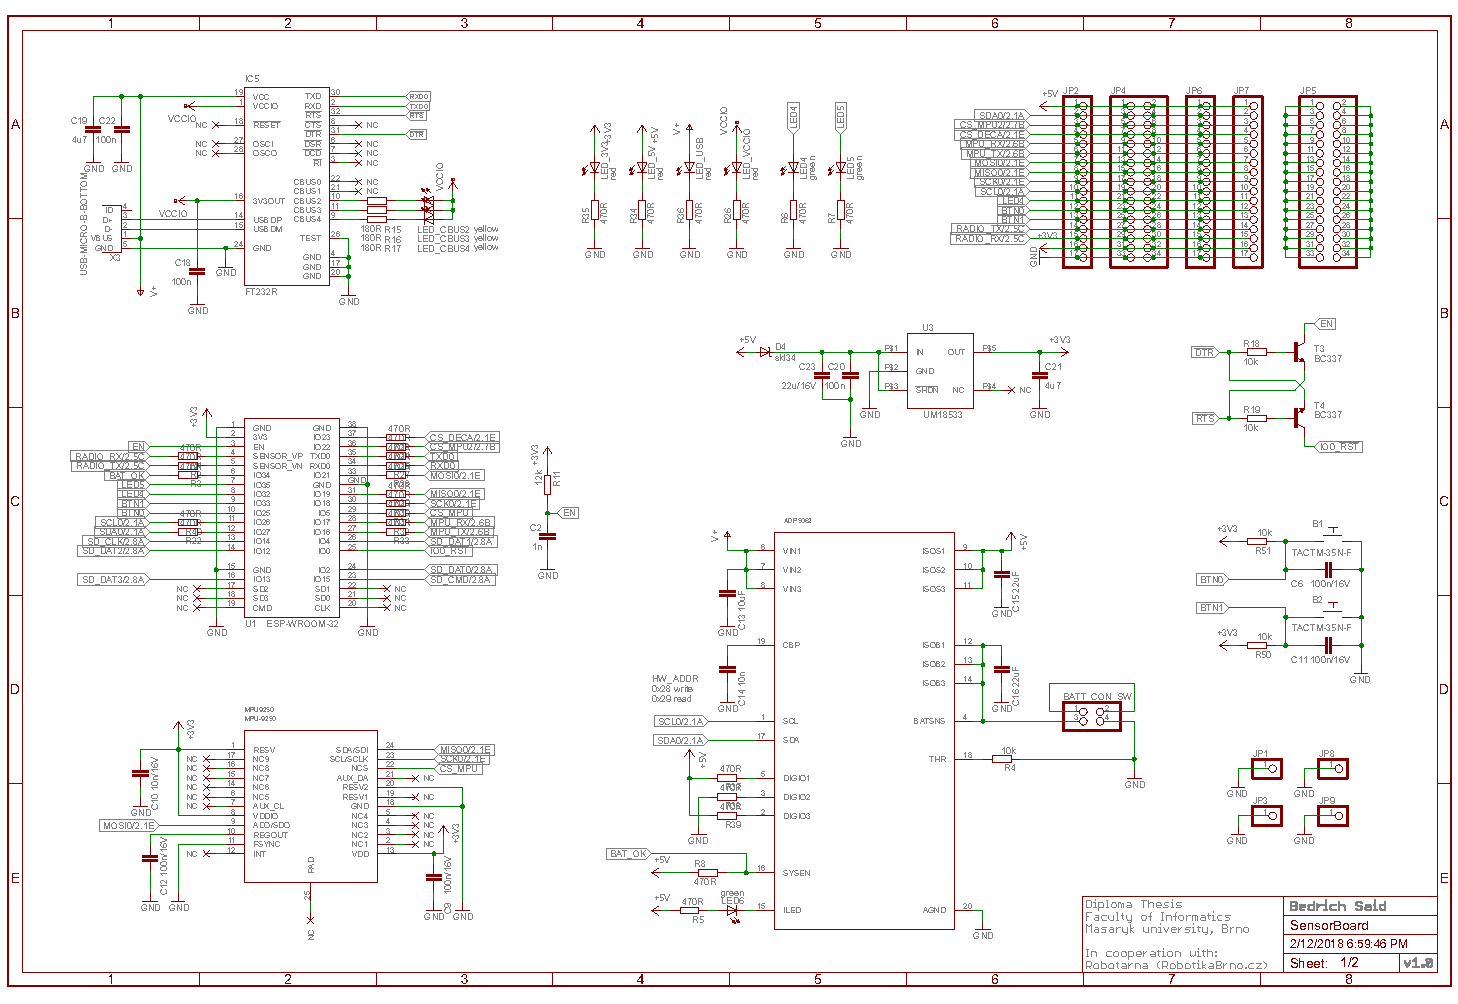
\includegraphics[angle=90, width=14cm]{img/sch1.pdf}
	\label{sch1}
	\caption{Schematics of the Sensor Board sheet 1}
\end{figure}

\begin{figure}
	\centering
	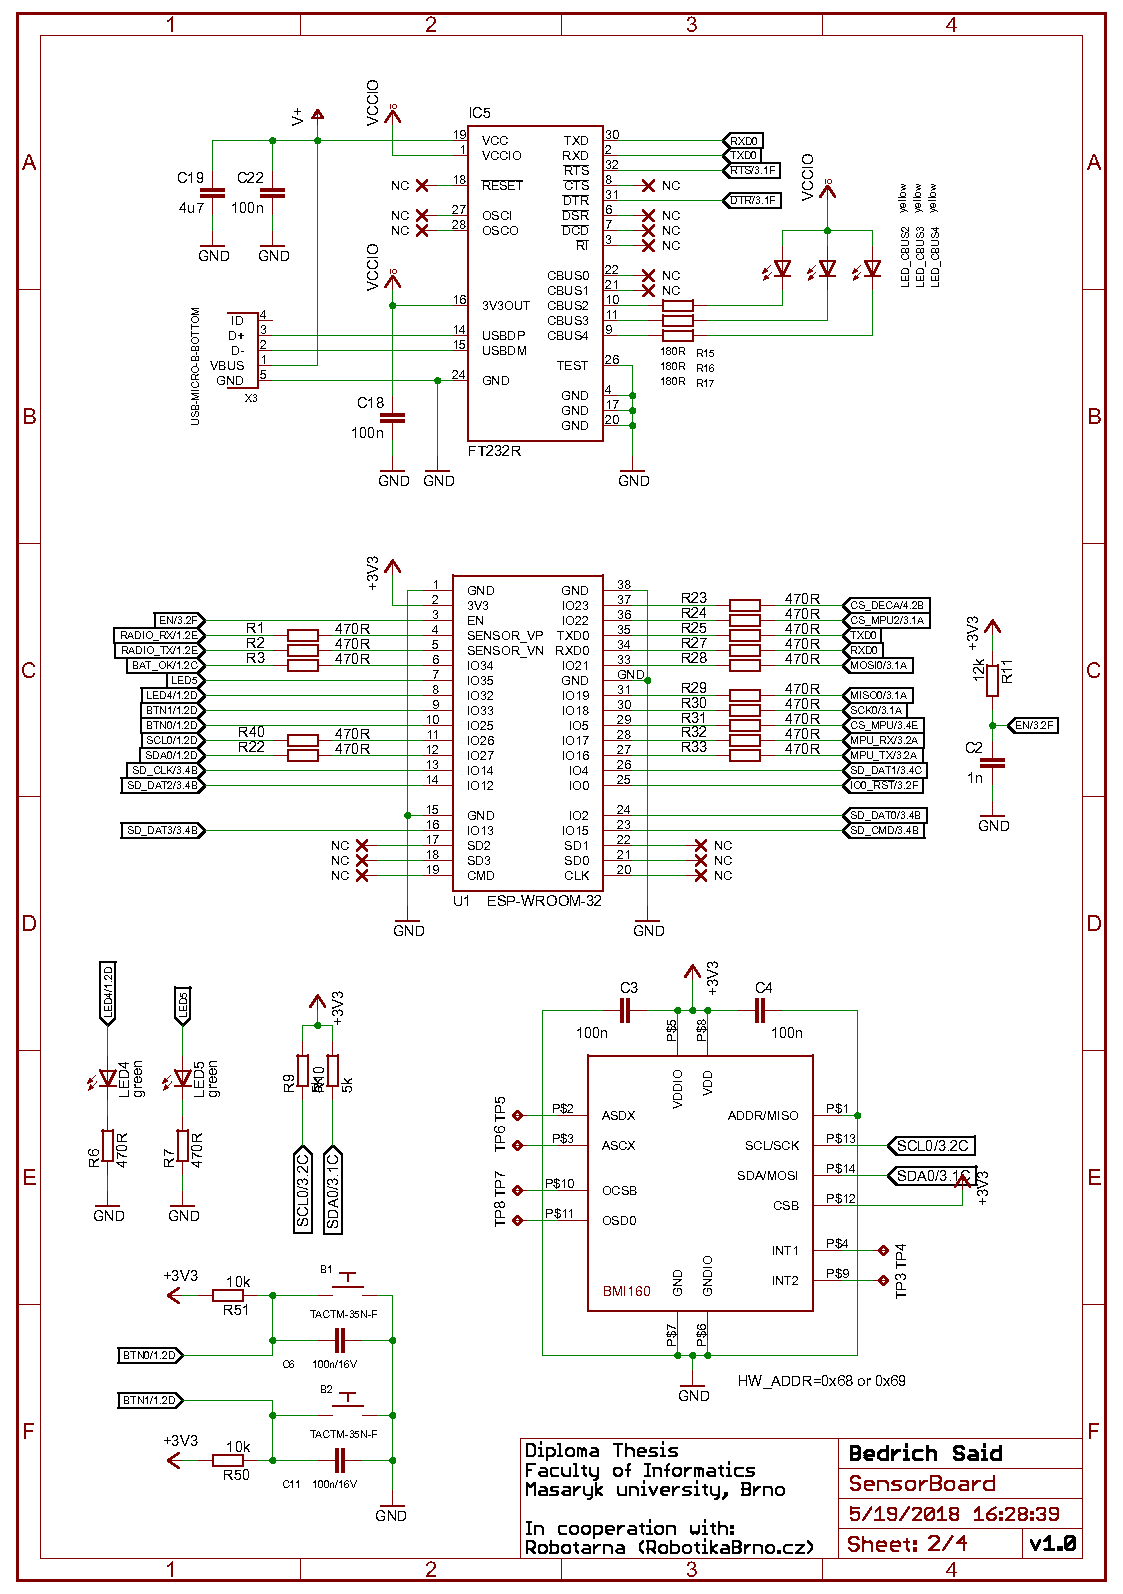
\includegraphics[angle=90, width=14cm]{img/sch2.pdf}
	\label{sch2}
	\caption{Schematics of the Sensor Board sheet 2}
\end{figure}

\begin{figure}
	\centering
	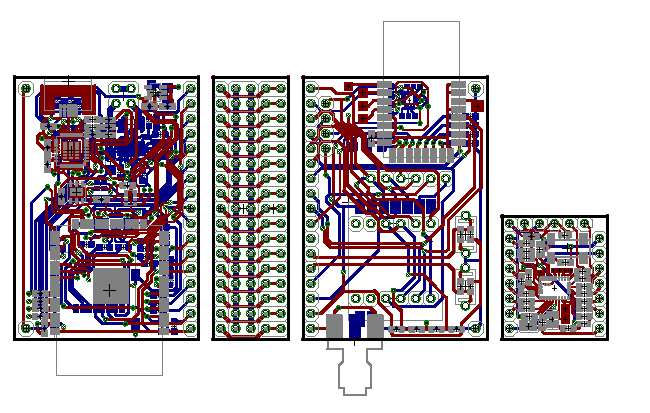
\includegraphics[scale=1]{img/brd.pdf}
	\vspace{-0.5cm}
	\begin{center}
		Top and Bottom layer
	\end{center}
	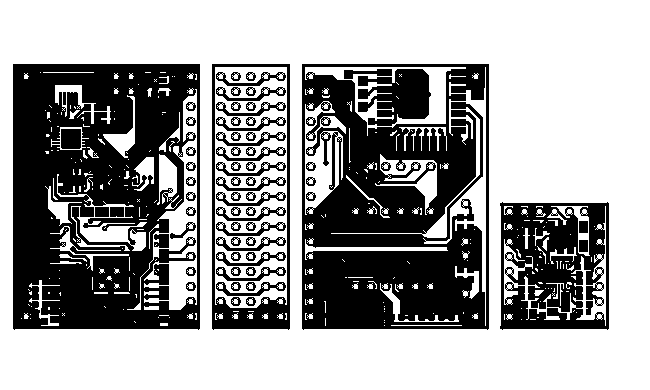
\includegraphics[scale=1]{img/brdTop.pdf}
	\vspace{-0.5cm}
	\begin{center}
		Only Top layer
	\end{center}
	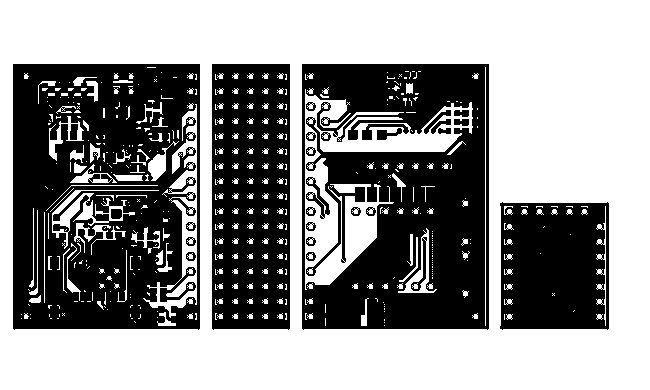
\includegraphics[scale=1]{img/brdBottom.pdf}
	\vspace{-0.5cm}
	\begin{center}
		Only Bottom layer
	\end{center}
	\label{brd1}
	\caption{Sensor Board layout in scale 1:1}
\end{figure}

\begin{figure}
	\centering
	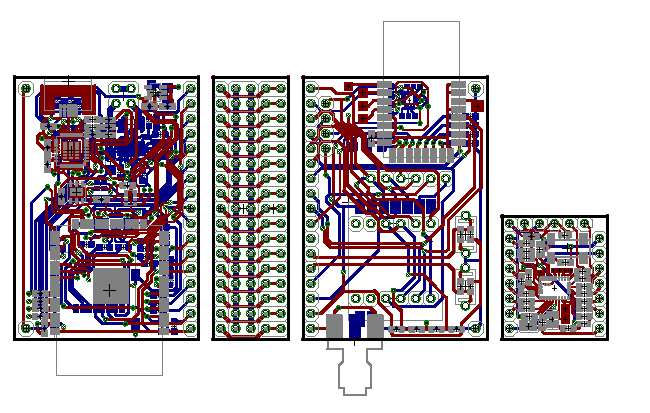
\includegraphics[angle=90, scale=2]{img/brd.pdf}
	\label{brd2}
	\caption{Sensor Board layout in detail scale 2:1}
\end{figure}

\subsection{Mechanical layout and connectors}
The mechanical layout is shown in figure \ref{fig:HWdimensions}.

\begin{figure}
	\centering
	\label{fig:HWdimensions}
	\caption{Sensor Board dimensions}
	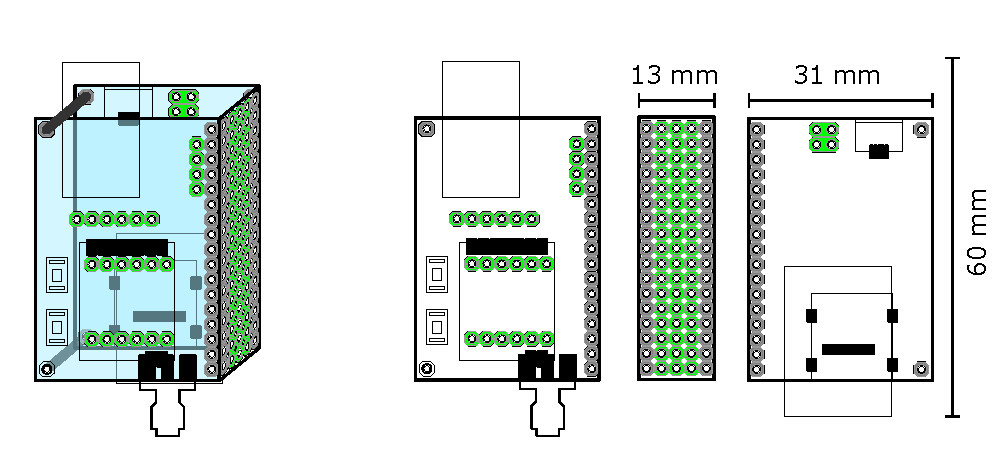
\includegraphics[scale=1]{img/HWdimensions.pdf}
\end{figure}

\section{Manufacturing}
\label{HWmanufacturing}

The manufacturing process of the prototype consists of these steps:
\begin{enumerate}
	\item Collecting source data -- schematics and board layout (in this paper in Eagle)
	\item Manufacturing of the Printed Circuit Board (\ac{PCB})
	\begin{enumerate}
		\item Panelization of the board layout
		\item Adding calibration markers
		\item Export gerber files
		\item Send exported files to manufacturing company
	\end{enumerate}
	\item Machine surface mount technology (\ac{SMT})
	\begin{enumerate}
		\item Export data for the template for applying solder paste
		\item Export partlist -- the list of all devices with their coordinates
		\item Export bill of materials (\ac{BOM})
		\item Manufacturing of the template for applying solder paste
		\item Order all devices according to \ac{BOM}
		\item Sending template for applying solder paste, packages with devices and part list to the manufacturer
	\end{enumerate}
	\item Finalization of the prototype
	\begin{enumerate}
		\item Hand soldering of some remaining devices like connectors or wires
		\item Completing the final prototype from possible parts and packaging
		\item Applying power and first testing
	\end{enumerate}
\end{enumerate}

\subsection{Collecting source data}
The source data may be in various formats according to the used tools. I used CadSoft \ac{EAGLE} \cite{EAGLE} during the development, but many other tools are available on the market. It depends on the manufacturer company if they accept the source data in our format. They usually accept the source data, but they usually apply an exporting fee. All \ac{PCB} editors should be able to export the manufacturing data in standardized formats. (Sometimes it's very hard or impossible to edit the exported data.)

\subsection{Manufacturing of the Printed Circuit Board}
When we have more than one board we should assemble all boards onto one or more panels. If we plan to solder the devices using the \ac{SMT}, we should add a calibration marks on the final panel. I have followed the instructions from SMTplus company \cite{SMTplusManual}.

First, I have panelized the separated boards and I have added the calibration marks according to the rules of SMTPlus company \cite{SMTPlusDesignRules}. Finally, I have exported the Gerber files using a CAM job \cite{GatemaCAMjob} in \ac{EAGLE}. I have followed the design rules for class 3 by Gatema a.s. company \cite{GatemaDesignRules}.

\subsection{Machine surface mount technology}
We need the \ac{PCB}, template for soldering paste and all devices in this step. Some \ac{PCB} manufacturers offer to create the template as well, so this is the way I used. The thickness of the template indicates the volume of the paste on each pad. For the small \ac{SMD} parts I used \SI{100}{\micro\meter}, but I recommend to discuss the parameters with the manufacturer.

The \ac{BOM} and part list export depends on the used design tools. When we connect used devices in the sources directly with their part numbers on selected shops, we can simply export the part list and then import it on the seller's website. I recommend buying some spare devices to minimize the risk of their damage.

\begin{figure}
	\centering
	\label{smtPasteTemplate}
	\caption{Template for soldering paste in scale 1:2}
	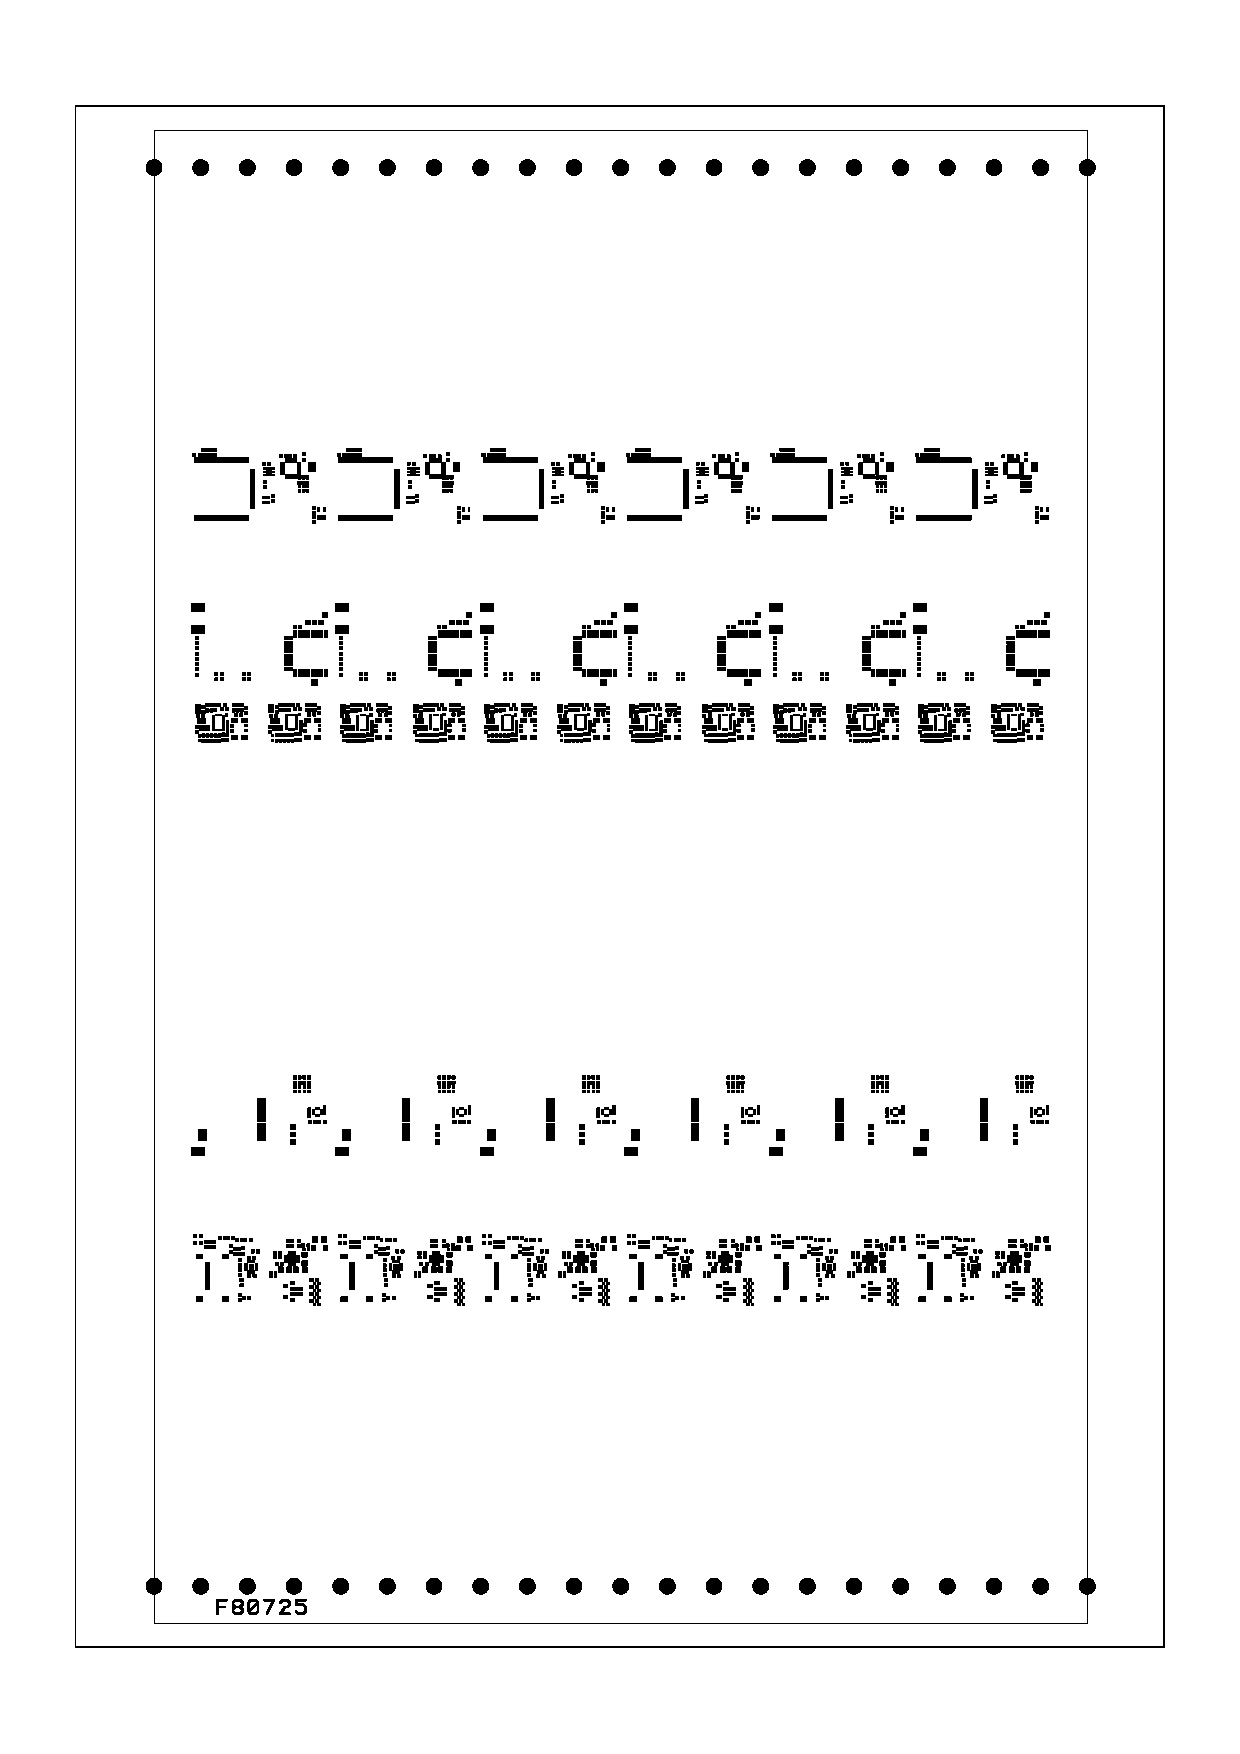
\includegraphics[angle=90, scale=0.5]{img/smtPasteTemplate.pdf}
\end{figure}

\subsection{Finalization of the prototype}
We can discuss the finalization works with the manufacturer, but when we create a prototype, I would like to recommend to do this job by yourself. It allows us to perform some tests before packaging and we don't have to spend time and money with a preparation of the documentation about how to assemble and package our prototype. Otherwise, the different software developers and testers can receive the different parts of the prototype for their next work.

\section{Testing}
\label{HWtesting}
The testing process has been split into two parts: the laboratory testing during the software development and the outdoor testing. I have found some errors in the version 1.0 during the laboratory testing. These errors are described in Errata list in section \ref{errata}. I did other tests against the specification of used devices. The results show us what devices should be used in the next version of the hardware and what devices are redundant. The results are shown in the section \ref{deviceTesting}. The outdoor tests didn't find any significant errors, but there were found several recommendations for the future versions of the SensorBoard. These recommendations are mentioned in section \ref{recommendationsNextVerison}.

\subsection{Errata}
\label{errata}
The tables \ref{tab:errata} and \ref{tab:errata2} show all errors I have found during software development and laboratory testing of the Sensor Board prototype.

\begin{table}
	\centering
	\caption{Errata of the SensorBoard}
	\label{tab:errata}
	\begin{tcolorbox}[tab2,tabularx={X|p{12cm}},title=Severity legend]
		\greenLow & No significant affects \\
		\greenSpare & Only spare devices may not work \\
		\yellowMedium & Some part of the prototype may not work \\
		\redHigh & The prototype has to be remade \\
	\end{tcolorbox}
	\vspace{1cm}
	\begin{tcolorbox}[tab2,tabularx={|c|p{7.5cm}|X|c|},title=Errata 1 of 2]
		Number & Description & Error created during & Severity \\ \hline
		1      &
		\parbox{7.5 cm}{\quad\\Bridge between boards under micro USB connector\\ \\ What happens:\\ The micro USB connector may be placed with lower accuracy\\}
		& panelization         & \greenLow      \\ \hline
		
		2      &
		\parbox{7.5 cm}{\quad\\Swapped MISO and MOSI on pins IO19 and IO21 on the ESP-WROOM-32 chip according to ESP32 Arduino standard\\ \\ What happens:\\ The SPI interface is not working in Arduino compatible mode without modification of the Arduino SPI library\\}
		& schematics design    & \yellowMedium   \\ \hline
		
		3      &
		\parbox{7.5 cm}{\quad\\LED5 connected to IO35 on ESP-WROOM-32 is not working\\ \\ What happens:\\ The pins IO34 -- IO39 are input only, so they cannot drive a LED\\}
		& schematics design    & \greenSpare    \\ \hline
		
		4      &
		\parbox{7.5 cm}{\quad\\Missing pull-up resistors on SD card\\ \\ What happens:\\ The SDIO interface needs external pull-up resistors to work properly. I have added these resistors later by hand.\\}
		& schematics design    & \yellowMedium   \\ \hline
	\end{tcolorbox}
\end{table}

\begin{table}
	\centering
	\caption{Errata of the SensorBoard}
	\label{tab:errata2}
	\begin{tcolorbox}[tab2,tabularx={|c|p{7.5cm}|X|c|},title=Errata 2 of 2]
		Number & Description & Error created during & Severity \\ \hline
		
		5      &
		\parbox{7.5 cm}{\quad\\The temperature measurement is placed very close to the main processor\\ \\ What happens:\\ The processor heating affects the measured temperature\\}
		& board layout         & \greenSpare    \\ \hline
		
		6      &
		\parbox{7.5 cm}{\quad\\Low capacity capacitor placed on power supply\\ \\ What happens:\\ When we use WiFi some brownouts can be detected. I have added a bigger capacitor later by hand.\\}
		& schematics design    & \yellowMedium   \\ \hline
		
		7      &
		\parbox{7.5 cm}{\quad\\The light sensor is placed on inner side of the board\\ \\ What happens:\\ The measured values are affected by shadow of the board.\\}
		& board layout         & \greenSpare    \\ \hline
		8      &
		\parbox{7.5 cm}{\quad\\Missing safety resistors on pins with buttons. These pins are directly connected to processor.\\ \\ What happens:\\ When the pins are defined in software to be used in different way, incorrect connection can burn the processor.\\}
		& schematics design        & \yellowMedium   \\ \hline
	\end{tcolorbox}
\end{table}

\subsection{Device testing}
\label{deviceTesting}
The device testing helped me to select the parts recommended for the future versions of the SensorBoard. It also helped me to mark all spare parts in the prototype. The table \ref{tab:deviceSelection} shows the results.

\begin{table}
	\centering
	\caption{Parts of the SensorBoard recommended for the future versions}
	\label{tab:deviceSelection}
	\begin{tcolorbox}[tab2,tabularx={X|p{12cm}},title=Decision legend]
		\greenCell{Selected} & Recommended for use in future versions \\ \hline
		\yellowCell{Possible} & Not necessary, but has use-cases, may be replaced with another part \\ \hline
		\redCell{Removed} & Not recommended or will be spare \\ \hline
	\end{tcolorbox}
	\vspace{1cm}
	\begin{tcolorbox}[tab2,tabularx={|X|p{7cm}|c|c|},title=Parts of the SensorBoard recommended for the future versions]
		Part ID & Description & Datasheet & Selected \\\hline\hline
		TACTM-35N-F & Button & \cite{TACTM} & \greenCell{Selected} \\
		ADP5062 & Power management and battery charger & \cite{analogdevices:ADP5062} & \greenCell{Selected} \\
		SI7006 & Humidity and temperature sensor & \cite{siliconlabs:SI7006} & \greenCell{Selected} \\
		DWM1000 & \ac{TDOA} location sensor (with antenna) & \cite{decawave:DWM1000} & \greenCell{Selected} \\
		BMP280 & Barometer & \cite{bosch:BMP280} & \greenCell{Selected} \\
		FT232R & UART to USB converter & \cite{ftdichip:FT232R} & \greenCell{Selected} \\
		MPU-9250 & Accelerometer, dynamic gyroscope, magnetometer & \cite{invensense:MPU9250} & \redCell{Removed} \\
		BMI160 & Accelerometer, dynamic gyroscope & \cite{bosch:BMI160} & \redCell{Removed} \\
		BMF055 & Accelerometer, dynamic gyroscope, magnetometer, ARM microcontroller & \cite{bosch:BMF055} & \greenCell{Selected} \\
		GY953 & Backup accelerometer, dynamic gyroscope and megnetometer with embedded pitch, roll and yaw angle estimation (sensor fusion) & \cite{GY953} & \redCell{Removed} \\
		HM-TRP & Long range \SI{433}{MHz} radio & \cite{HM-TRP} & \yellowCell{Possible} \\
		MOLEX-47219-2001 & Micro SD card holder & \cite{MOLEX-SD1} & \greenCell{Selected} \\
		LTR-329ALS & Digital ambient light sensor & \cite{LTR-329ALS} & \greenCell{Selected} \\
		ESP-WROOM-32 & Dual core controller with WiFi and Bluetooth & \cite{espressif:ESP-WROOM-32} & \greenCell{Selected} \\
		UM18533 & \parbox{7 cm}{Linear stabilizer \SI{3.3}{V} \\\\ Note: Insufficient current} & \cite{UM18533} & \redCell{Removed} \\
		LF33 & Linear stabilizer \SI{3.3}{V} & \cite{LF33} & \greenCell{Selected} \\
		USB-MICRO & Micro USB connector & \cite{USB-MICRO} & \greenCell{Selected} \\
		Pin header 2.54 mm & Servo connector & \cite{PINHEAD} & \yellowCell{Possible} \\
	\end{tcolorbox}
\end{table}

\subsection{Recommendations for the next version}
\label{recommendationsNextVerison}
Recommendations for the future versions of the Sensor Board based on the outdoor testing:
\begin{itemize}
	\item[--] Replace software LEDs by one or more RGB LEDs. For example WS2812 RGB LED \cite{AdafruitLED}.
	\item[--] Move the sensor fusion and computations to Atmel SAM D21 \cite{AtmelSAM} processor inside the BMF055 \cite{BMF055} chip. Keep the ESP32 \cite{ESP32} processor only for communication and user computations.
	\item[--] Decrease board dimensions using 4 layer \ac{PCB}. The increased cost for 4 layer board may be saved on a smaller surface.
	\item[--] Sometimes it is better to have all \ac{SMD} parts on one side of the board. The manufacturing is cheaper and the space on the second side can be used for example for battery mounting or for connectors.
	\item[--] Split the board area to an area for sensors, an area for power electronics and an area for computing. The power distribution is easier in this situation and the sensors are less influenced by other electronics.
	\item[--] Use another driver with more capabilities for USB connection. The USB on board actually supports only UART communication on the virtual COM port. The File Transfer protocol for the SD card should be supported, too. (If it is needed we can add full USB host support or USB-C compatibility.)
	\item[--] Add specialized pads for an oscilloscope. The pads are connected to the signal and to the ground, so the oscilloscope measurements are more accurate.
	\item[--] The main processor should be able to switch on/off the power of other parts (sensors). The sensors support sleep modes, but we cannot completely switch them off to save more energy from the battery.
	\item[--] If we recognize that the ESP-WROOM-32 controller is not powerful enough, we can use a fully compatible alternative with larger memory ALB32-WROVER \cite{ALB32-WROVER}. It should be possible to compile a terminal based Linux distribution for this controller.
\end{itemize}

\subsection{Analysis of additional costs}
\label{HWadditionalCosts}
By the analysis of additional costs, I mean the counting the prices of all parts that were finally spare or weren't used. The table \ref{tab:additionalCost} counts all parts of the SensorBoard and their prices.

The column "Used" tells us if the item was used for any use case or if it was spare at all times. If any item is still unused it doesn't mean that it cannot be used in some future use case. The column "Is necessary" points the basic items, the SensorBoard can't work or can't be built without them.

It means that the green cost "Total used and necessary" is the lowest cost of the prototype without any additional functionality. The yellow cost "Total used and unnecessary" is the cost of all items that had significant value during development, but weren't mandatory for the main task. These items also made the development process easier and faster, so I don't count this cost as additional. The last red cost "Total unused" covers all items that weren't used. These items were a part of the design because they lowered some risks in functionality. For example, if I wasn't sure that an accelerometer will work properly, I added another spare accelerometer, which covered this risk. I could get a working prototype in the first iteration using this strategy. I finally count the red cost as a cost of decreased risks and as a cost of higher versatility.

We have to take into account that all the mentioned costs are costs of the prototype. The same items would have significantly lower costs during the production of more devices.

\begin{table}
	\centering
	\caption{Additional cost calculation}
	\label{tab:additionalCost}
	\begin{tcolorbox}[tab2,tabularx={|X|l|c|c|},title=Additional cost calculation]
		Part ID & Price & Used & Is necessary \\\hline\hline
		\ac{PCB} & \$ 23 & \greenYes & \greenYes \\
		\ac{SMT} job & \$ 65 & \greenYes & \greenYes \\ \hline
		TACTM-35N-F & \$ 0.4 & \greenYes & \yellowCell{No} \\
		ADP5062 & \$ 3.8 & \greenYes & \greenYes \\
		SI7006 & \$ 2 & \redNo & \redNo \\
		DWM1000 & \$ 22 & \greenYes & \yellowCell{No} \\
		BMP280 & \$ 4 & \greenYes & \yellowCell{No} \\
		FT232R & \$ 5 & \greenYes & \greenYes \\
		MPU-9250 & \$ 10 & \greenYes & \yellowCell{No} \\
		BMI160 & \$ 4.3 & \redNo & \redNo \\
		BMF055 & \$ 11 & \greenYes & \greenYes \\
		GY953 & \$ 11 & \redNo & \redNo \\
		HM-TRP & \$ 13 & \greenYes & \yellowCell{No}\\
		MOLEX-47219-2001 & \$ 1.2 & \greenYes & \greenYes \\
		LTR-329ALS & \$ 0.7 & \redNo & \redNo \\
		ESP-WROOM-32 & \$ 12 & \greenYes & \greenYes \\ \hline \hline
		\greenCell{\textbf{Total used and necessary}} & \greenCell{\textbf{\$ 121}} & \greenYes & \greenYes \\
		\yellowCell{\textbf{Total used and unnecessary}} & \yellowCell{\textbf{\$ 49.4}} & \yellowCell{Yes} & \yellowCell{No} \\
		\redCell{\textbf{Total unused}} & \redCell{\textbf{\$ 18}} & \redNo & \redNo \\
	\end{tcolorbox}
\end{table}

\chapter{Conclusion}
The work was finally split into four milestones. The first milestone was achieved when I have decided to develop a new data logging hardware, because the existing solutions didn't fulfilled all the requirements. I have successfully developed the SensorBoard hardware in the second step and then the board was manufactured in six copies. I have achieved the second milestone with the manufactured hardware. The third phase was about testing the hardware and about implementing libraries for communication between the controller and other parts, mainly sensors. I have found several mistakes in the hardware design during programming, but all of them were corrected. The third milestone was achieved when I had a working hardware with C++ libraries for easier communication with sensors and other parts of the hardware. These libraries are a part of the API. During the last phase I have implemented the firmware for real-time movement analysis. When the SensorBoard is placed on a horse under the saddle, it is able to recognize the kind of movement of a horse. This firmware demonstrates the functionality of the designed hardware in real use. I have achieved the last milestone during the first successful test of the platform on a horse's body.

There are many applications and use cases of the SensorBoard presented as examples in the thesis. I have selected the movement analysis case, because this task started the whole project in the begining. The movement analysis firmware shows the advantages of running some user code on the hardware. We can see the results of the analysis in real-time.

If there is an interest on future work with this hardware, I would recommend to create the second version of the SensorBoard with attention to the list of hardware errors presented in this thesis. The SensorBoard was used for example as a simple autopilot of a small quadcopter, so I believe that it will be used in several applications in the near future. I hope that the firmware for the movement analysis of a horse will help to work with this kind of animals easier.

\end{document}
